% !TEX root = main.tex
\documentclass[12pt,a4paper]{report}
\usepackage{hyperref}
\usepackage{url}
\usepackage{amsmath}
\usepackage{amssymb}
\usepackage{graphicx}
\usepackage{booktabs}
\usepackage{caption}
\usepackage{subcaption}
\usepackage{csquotes}
\usepackage{xcolor}
\usepackage{listings}
% Temporarily commenting out unavailable packages
% \usepackage{algorithm}
% \usepackage{algpseudocode}
% \usepackage{physics}
\usepackage{microtype}
\usepackage[margin=1in]{geometry}
\usepackage[
backend=biber,
style=alphabetic,
bibstyle=reading,
sorting=nyt
]{biblatex}

% Configure hyperref for better PDF navigation
\hypersetup{
    colorlinks=true,
    linkcolor=blue,
    filecolor=magenta,
    urlcolor=cyan,
    pdftitle={Quantum Computing and Its Impact on Cryptography},
    pdfauthor={Lou Sergonne}
}

% Configure graphicx to look for images in the src/images directory
\graphicspath{{src/images/}}

\addbibresource{src/bibliography/bibliography.bib}
\title{\LARGE{\textbf{Quantum Computing and Its Impact on Cryptography}}}
\author{\Large{Lou Sergonne}}
\date{2024-2025}

\begin{document}

\maketitle
\tableofcontents

\chapter{Introduction}\label{chap:introduction}

Quantum computers are changing the world of online security. This memoire looks at two main things: how quantum computers can break current security methods, and what we can do to stay secure in the future.

Our online world relies on security systems (cryptography) that are designed to be too hard for regular computers to crack. But quantum computers are different. They are much more powerful for certain tasks and can break many of these security systems.

\includegraphics[width=0.8\textwidth]{01_Introduction/quantum_vs_classical}

This quantum threat is a big deal because:
\begin{itemize}
    \item Our current online security might not work against quantum computers.
    \item We urgently need to find new security methods that can resist quantum computers.
    \item Quantum technology itself might also offer new ways to keep things secure.
\end{itemize}

\section{Structure of this Memoire}

This paper is organized chapter by chapter:
\begin{itemize}
    \item \textbf{Chapter 2: Basics of Quantum Computing} --- Explains the core ideas of quantum computing
    \item \textbf{Chapter 3: Regular vs. Quantum Computing} --- Compares regular and quantum computers and why this matters for security
    \item \textbf{Chapter 4: How Current Security Works} --- Reviews the security methods we use today and how they are supposed to be secure
    \item \textbf{Chapter 5: Quantum Threats to Security} --- Explains exactly how quantum computers can break current security systems
    \item \textbf{Chapter 6: Making the Change} --- Looks at the challenges of switching to new, quantum-resistant security systems
    \item \textbf{Chapter 7: New Security Methods} --- Explores security solutions that should work even against quantum computers
    \item \textbf{Chapter 8: What's Next?} --- Considers future developments and trends in this area \parencite{preskill2018quantum}
    \item \textbf{Chapter 9: Impact on Society} --- Discusses the wider effects of these changes beyond just technology
\end{itemize}
\chapter{Fundamentals of Quantum Computing}\label{chap:fundamentals}

\section{Quantum Mechanics Principles}\label{sec:quantum_principles}

The foundation of quantum computing rests on several key quantum mechanical principles:

\subsection{Superposition}\label{subsec:superposition}
In quantum mechanics, a system can exist in multiple states simultaneously until measured. Mathematically, a quantum state $|\psi\rangle$ of a single qubit can be expressed as:
\begin{equation}\label{eq:superposition}
    |\psi\rangle = \alpha|0\rangle + \beta|1\rangle
\end{equation}
where $|0\rangle$ and $|1\rangle$ are the computational basis states (analogous to classical bits 0 and 1), and $\alpha$ and $\beta$ are complex numbers called probability amplitudes. The squares of their absolute values represent the probabilities of measuring the qubit in the corresponding basis state, satisfying $|\alpha|^2 + |\beta|^2 = 1$. This ability to exist in a combination of states allows quantum computers to explore many possibilities concurrently.

\subsection{Quantum Bits}\label{subsec:qubits}
Unlike classical bits which can only be 0 or 1, quantum bits (qubits) can exist in a superposition of both states, as described above. This property is often visualized using the Bloch sphere (Figure~\ref{fig:bloch_sphere}), where any point on the surface of the sphere represents a possible pure state of a single qubit.

\begin{figure}[h]
    \centering
    % Ensure the image path is correct relative to the main.tex file
    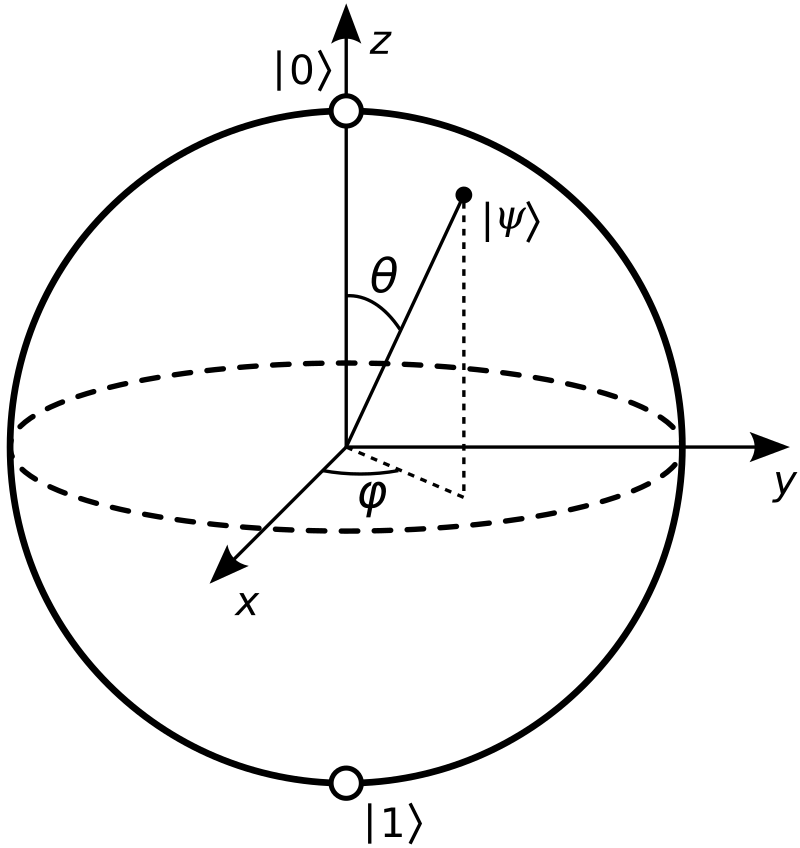
\includegraphics[width=0.6\textwidth]{02_Fundamentals_of_Quantum_Computing/bloch_sphere}
    \caption{The Bloch sphere representation of a single qubit state $|\psi\rangle = \cos(\theta/2)|0\rangle + e^{i\phi}\sin(\theta/2)|1\rangle$. The north pole represents $|0\rangle$, the south pole $|1\rangle$.}
    \label{fig:bloch_sphere}
\end{figure}

\subsubsection*{Physical Implementations}
Realizing qubits physically presents diverse approaches, each with unique advantages and challenges:
\begin{itemize}
    \item \textbf{Superconducting Circuits:} Utilize circuits with Josephson junctions cooled to milli-Kelvin temperatures. These allow for fast gate operations (nanoseconds) and are a leading technology, but require significant cryogenic infrastructure and are sensitive to noise.
    \item \textbf{Trapped Ions:} Individual charged atoms confined by electromagnetic fields. They boast very long coherence times (seconds to minutes) and high gate fidelities, but gate operations are typically slower (microseconds).
    \item \textbf{Photonic Qubits:} Employ quantum states of light (e.g., polarization or path encoding). Photons are naturally robust against decoherence and ideal for communication (Quantum Key Distribution), but building universal quantum gates for computation is challenging.
    \item \textbf{Other Platforms:} Include neutral atoms, quantum dots, topological qubits, and NV-centers in diamond, each representing active areas of research.
\end{itemize}
A major engineering challenge common to all platforms is maintaining quantum coherence—preserving the delicate superposition and entanglement against environmental noise (e.g., thermal fluctuations, stray electromagnetic fields) which causes decoherence (loss of quantum information). This necessitates sophisticated control systems, shielding, and often, operation at extremely low temperatures or high vacuum.

\subsection{Entanglement}\label{subsec:entanglement}
Quantum entanglement is a unique quantum correlation where two or more qubits become linked in such a way that they share the same fate, regardless of the distance separating them. Their states are described by a single, combined quantum state, not independent individual states. For example, if two qubits are entangled in the Bell state:
\begin{equation*}
    |\Phi^+\rangle = \frac{1}{\sqrt{2}}(|00\rangle + |11\rangle)
\end{equation*}
measuring the first qubit to be $|0\rangle$ instantly forces the second qubit to be $|0\rangle$, and measuring the first as $|1\rangle$ forces the second to be $|1\rangle$, even if they are light-years apart. This correlation, famously dubbed "spooky action at a distance" by Einstein, cannot be explained by classical physics (e.g., hidden variables) and is experimentally verified. While entanglement does not allow faster-than-light communication (information transfer still requires classical communication), it is a crucial resource enabling quantum algorithms (like Shor's), quantum teleportation, and certain quantum cryptographic protocols.

\section{Quantum Gates and Circuits}\label{sec:quantum_gates}

Quantum computations are performed by applying sequences of \textbf{quantum gates} to qubits. These gates are analogous to classical logic gates but operate on quantum states. Mathematically, single-qubit gates are represented by $2 \times 2$ unitary matrices ($U^\dagger U = I$), and multi-qubit gates by larger unitary matrices, ensuring that the evolution of quantum states is reversible and preserves probabilities. Below are examples of important quantum gates:

\subsection*{Pauli-X (NOT) Gate}
The Pauli-X gate acts as a quantum bit-flip, analogous to the classical NOT gate. It transforms $|0\rangle$ to $|1\rangle$ and $|1\rangle$ to $|0\rangle$. For a general qubit $|\psi\rangle = \alpha|0\rangle + \beta|1\rangle$:
\begin{equation*}
    X|\psi\rangle = X(\alpha|0\rangle + \beta|1\rangle) = \alpha|1\rangle + \beta|0\rangle
\end{equation*}
Matrix form:
\begin{equation*}
    X = \begin{pmatrix} 0 & 1 \\ 1 & 0 \end{pmatrix}
\end{equation*}

\subsection*{Pauli-Y Gate}
The Pauli-Y gate performs a bit-flip combined with phase changes.
\begin{equation*}
    Y|\psi\rangle = Y(\alpha|0\rangle + \beta|1\rangle) = \alpha(i|1\rangle) + \beta(-i|0\rangle) = -i\beta|0\rangle + i\alpha|1\rangle
\end{equation*}
Matrix form:
\begin{equation*}
    Y = \begin{pmatrix} 0 & -i \\ i & 0 \end{pmatrix}
\end{equation*}

\subsection*{Pauli-Z Gate}
The Pauli-Z gate acts as a phase-flip, leaving $|0\rangle$ unchanged and mapping $|1\rangle$ to $-|1\rangle$.
\begin{equation*}
    Z|\psi\rangle = Z(\alpha|0\rangle + \beta|1\rangle) = \alpha|0\rangle - \beta|1\rangle
\end{equation*}
Matrix form:
\begin{equation*}
    Z = \begin{pmatrix} 1 & 0 \\ 0 & -1 \end{pmatrix}
\end{equation*}

\subsection*{Hadamard (H) Gate}
The Hadamard gate is crucial for creating superposition. It transforms $|0\rangle$ into an equal superposition of $|0\rangle$ and $|1\rangle$, and $|1\rangle$ into an equal superposition with a phase difference.
\begin{equation*}
    H|0\rangle = \frac{|0\rangle + |1\rangle}{\sqrt{2}}, \quad H|1\rangle = \frac{|0\rangle - |1\rangle}{\sqrt{2}}
\end{equation*}
Applying H twice returns the original state ($H^2 = I$).
Matrix form:
\begin{equation*}
    H = \frac{1}{\sqrt{2}}\begin{pmatrix} 1 & 1 \\ 1 & -1 \end{pmatrix}
\end{equation*}

\subsection*{Phase (S or $\sqrt{Z}$) Gate}
The S gate introduces a relative phase shift of $\pi/2$ (or $i$) between the $|0\rangle$ and $|1\rangle$ components. It is sometimes called the $\sqrt{Z}$ gate as $S^2 = Z$.
\begin{equation*}
    S|\psi\rangle = S(\alpha|0\rangle + \beta|1\rangle) = \alpha|0\rangle + i\beta|1\rangle
\end{equation*}
Matrix form:
\begin{equation*}
    S = \begin{pmatrix} 1 & 0 \\ 0 & i \end{pmatrix}
\end{equation*}

\subsection*{T (or $\pi/8$) Gate}
The T gate introduces a relative phase shift of $\pi/4$. It is important because H, S, and CNOT gates alone are not sufficient for universal quantum computation; adding the T gate completes a common universal set.
\begin{equation*}
    T|\psi\rangle = T(\alpha|0\rangle + \beta|1\rangle) = \alpha|0\rangle + e^{i\pi/4}\beta|1\rangle
\end{equation*}
Matrix form:
\begin{equation*}
    T = \begin{pmatrix} 1 & 0 \\ 0 & e^{i\pi/4} \end{pmatrix} = \begin{pmatrix} 1 & 0 \\ 0 & \frac{1+i}{\sqrt{2}} \end{pmatrix}
\end{equation*}

\subsection*{CNOT (Controlled-NOT) Gate}
The CNOT gate is a fundamental two-qubit gate. It flips the state of the second qubit (target) if and only if the first qubit (control) is in the state $|1\rangle$.
\begin{align*}
    \text{CNOT}|00\rangle &= |00\rangle \\
    \text{CNOT}|01\rangle &= |01\rangle \\
    \text{CNOT}|10\rangle &= |11\rangle \\
    \text{CNOT}|11\rangle &= |10\rangle
\end{align*}
Matrix form (acting on basis states $|00\rangle, |01\rangle, |10\rangle, |11\rangle$):
\begin{equation*}
    \text{CNOT} = \begin{pmatrix} 1 & 0 & 0 & 0 \\ 0 & 1 & 0 & 0 \\ 0 & 0 & 0 & 1 \\ 0 & 0 & 1 & 0 \end{pmatrix}
\end{equation*}
The CNOT gate is essential for creating entanglement and is a key component in many quantum algorithms and error correction codes.

\subsection*{Toffoli (CCNOT) Gate}
The Toffoli gate is a three-qubit gate, acting as a controlled-controlled-NOT. It flips the third qubit if and only if the first two control qubits are both in the state $|1\rangle$.
\begin{equation*}
    \text{CCNOT}|abc\rangle = |ab(c\oplus(a\cdot b))\rangle
\end{equation*}
where $\oplus$ is addition modulo 2.
Matrix form (acting on basis states $|000\rangle$ through $|111\rangle$):
\begin{equation*}
    \text{CCNOT} = \begin{pmatrix}
    1&0&0&0&0&0&0&0 \\
    0&1&0&0&0&0&0&0 \\
    0&0&1&0&0&0&0&0 \\
    0&0&0&1&0&0&0&0 \\
    0&0&0&0&1&0&0&0 \\
    0&0&0&0&0&1&0&0 \\
    0&0&0&0&0&0&0&1 \\ % Flips |110> to |111>
    0&0&0&0&0&0&1&0  % Flips |111> to |110>
    \end{pmatrix}
\end{equation*}
The Toffoli gate is universal for classical reversible computation. Together with the Hadamard gate (or other suitable single-qubit rotations), it forms a universal set for quantum computation, meaning any quantum computation can be decomposed into a sequence of these gates.

\subsection*{Bell States Creation}
Applying a Hadamard gate to the first qubit (initially $|0\rangle$) followed by a CNOT gate controlled by the first qubit acting on the second (initially $|0\rangle$) creates the Bell state $|\Phi^+\rangle$:
\begin{enumerate}
    \item Start with $|00\rangle$.
    \item Apply H to the first qubit: $H|0\rangle \otimes |0\rangle = \frac{1}{\sqrt{2}}(|0\rangle + |1\rangle) \otimes |0\rangle = \frac{1}{\sqrt{2}}(|00\rangle + |10\rangle)$.
    \item Apply CNOT (control=1st, target=2nd): $\text{CNOT} \left( \frac{1}{\sqrt{2}}(|00\rangle + |10\rangle) \right) = \frac{1}{\sqrt{2}}(|00\rangle + |11\rangle) = |\Phi^+\rangle$.
\end{enumerate}
This maximally entangled state demonstrates how quantum gates can generate non-classical correlations essential for quantum algorithms.

\section{Quantum Algorithms}\label{sec:quantum_algorithms}

Quantum algorithms leverage the principles of superposition, entanglement, and quantum interference to perform computations in ways that can dramatically outperform classical algorithms for specific problems. This section introduces three cornerstone quantum algorithms: the Quantum Fourier Transform (QFT), Quantum Phase Estimation (QPE), and Amplitude Amplification (which generalizes Grover's search algorithm), highlighting their mechanisms, interdependencies, and cryptographic relevance.

\subsection{Quantum Fourier Transform (QFT)}\label{subsec:qft}
The Quantum Fourier Transform (QFT) is the quantum analogue of the classical Discrete Fourier Transform (DFT). It maps a quantum state represented in the computational basis to its representation in the Fourier basis. Its primary strength lies in efficiently finding periodicities in quantum states.

When applied to a computational basis state $|j\rangle$ (where $j$ is an integer represented by $n$ qubits), the QFT generates a superposition state:
\begin{equation}\label{eq:qft}
    \text{QFT}|j\rangle = \frac{1}{\sqrt{N}} \sum_{k=0}^{N-1} e^{2\pi i jk/N} |k\rangle
\end{equation}
where $N=2^n$ is the dimension of the state space. While a classical Fast Fourier Transform (FFT) takes $\mathcal{O}(N\log N)$ operations, the QFT circuit can be implemented using only $\mathcal{O}(n^2) = \mathcal{O}((\log N)^2)$ quantum gates (Hadamard and controlled phase rotations $R_m$), offering an exponential speedup in terms of $n$.

\begin{figure}[h]
    \centering
    % Ensure the image path is correct relative to the main.tex file
    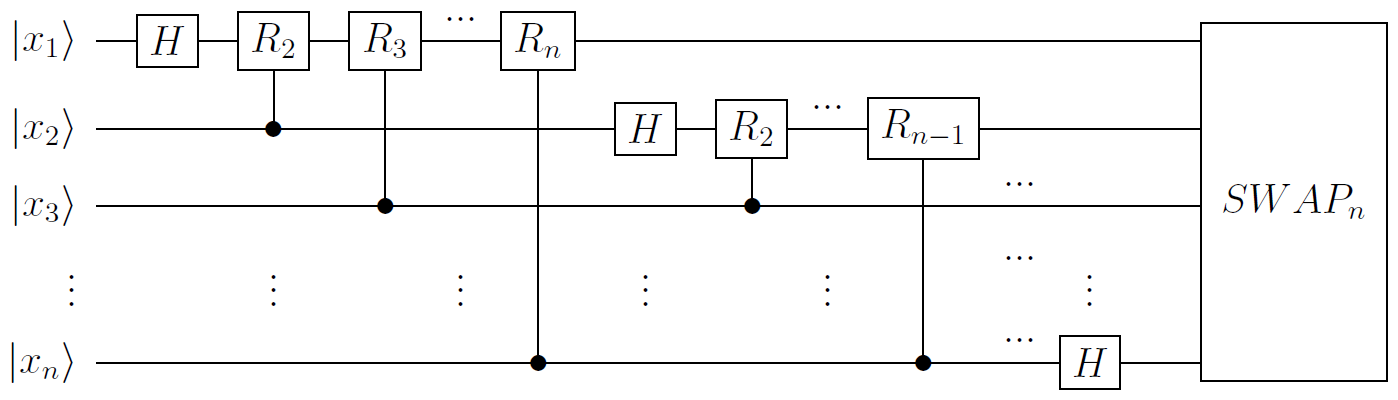
\includegraphics[width=0.8\textwidth]{02_Fundamentals_of_Quantum_Computing/qft_circuit}
    \caption{Quantum circuit implementing the QFT using layered Hadamard gates (H) and controlled phase rotations ($R_m$). Qubit ordering typically assumes $|x_1\rangle$ is the most significant qubit and $|x_n\rangle$ the least significant.}
    \label{fig:qft_circuit}
\end{figure}

The phase rotation gates $R_m$ are defined by:
\begin{equation}\label{eq:phase_gate}
    R_m = \begin{pmatrix} 1 & 0 \\ 0 & e^{2\pi i /2^m} \end{pmatrix}
\end{equation}
These gates apply progressively smaller phase shifts.

\textbf{Cryptographic Relevance:} The QFT's ability to efficiently find periods is the core component enabling \textbf{Shor's algorithm} to factor large integers and compute discrete logarithms exponentially faster than the best known classical algorithms. Shor's algorithm uses the QFT to find the period of the modular exponentiation function $f(x) = a^x \bmod N$, which then allows efficient calculation of the factors of $N$ or the discrete logarithm.

\subsection{Quantum Phase Estimation (QPE)}\label{subsec:qpe}
Quantum Phase Estimation is a fundamental quantum algorithm used to determine the eigenvalue (specifically, the phase) of an eigenvector of a unitary operator. Given a unitary operator $U$ and one of its eigenstates $|\psi\rangle$ such that $U|\psi\rangle = e^{2\pi i\theta}|\psi\rangle$, QPE efficiently estimates the phase $\theta \in [0, 1)$.

The algorithm uses two registers: the first (measurement register) with $m$ qubits initialized to $|0\rangle^{\otimes m}$, and the second (target register) initialized to the eigenstate $|\psi\rangle$.
Key steps:
\begin{enumerate}
    \item Apply Hadamard gates to the first register: $\frac{1}{\sqrt{2^m}}\sum_{k=0}^{2^m-1}|k\rangle \otimes |\psi\rangle$.
    \item Apply controlled-$U^{2^j}$ operations (controlled by the $j$-th qubit of the first register) to the second register. This encodes the phase $\theta$ into the first register's state: $\frac{1}{\sqrt{2^m}} \sum_{k=0}^{2^m-1} e^{2\pi i\theta k} |k\rangle \otimes |\psi\rangle$.
    \item Apply the inverse Quantum Fourier Transform (QFT$^{-1}$) to the first register.
    \item Measure the first register. The measurement outcome provides an $m$-bit approximation of $\theta$.
\end{enumerate}
The precision of the estimate scales as $2^{-m}$.

\begin{figure}[h]
\centering
 % Ensure the image path is correct relative to the main.tex file
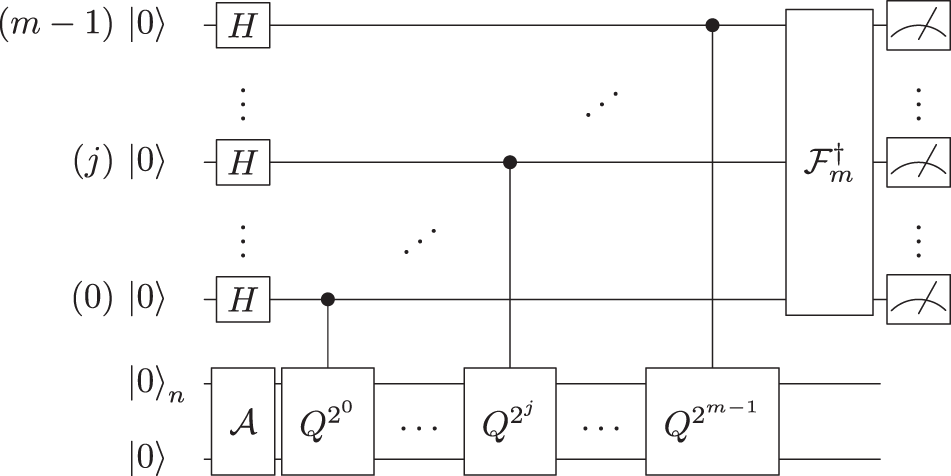
\includegraphics[width=0.8\textwidth]{02_Fundamentals_of_Quantum_Computing/qpe_circuit}
\caption{Quantum circuit for Phase Estimation. The top $m$ qubits form the measurement register, the bottom $n$ qubits hold the eigenstate $|\psi\rangle$. QFT$^{-1}$ is the inverse Quantum Fourier Transform.}
\label{fig:qpe_circuit}
\end{figure}

\textbf{Cryptographic Relevance:} QPE is the subroutine within \textbf{Shor's algorithm} that actually extracts the period information. The modular exponentiation operation can be implemented as a unitary operator $U$, and QPE is used to estimate the phase related to its eigenvalues, which in turn reveals the period needed for factoring or solving the discrete logarithm problem.

\subsection{Amplitude Amplification (Grover's Algorithm)}\label{subsec:amplitude_amp}
Amplitude Amplification is a general quantum technique for boosting the probability of measuring a desired ('good' or 'marked') state from a superposition. \textbf{Grover's search algorithm} is the most famous application, designed to find a specific item in an unsorted database (or search space) of size $N$.

Classically, finding the marked item requires, on average, $N/2$ queries (and $N$ in the worst case). Grover's algorithm achieves this with only $\mathcal{O}(\sqrt{N})$ quantum queries, providing a quadratic speedup. It doesn't offer the exponential speedup of Shor's algorithm but is applicable to a wider range of problems.

The algorithm works by iteratively rotating the quantum state vector towards the 'good' state(s). Suppose an initial state $|\psi\rangle$ is a superposition of 'good' states $|G\rangle$ and 'bad' states $|B\rangle$: $|\psi\rangle = \sin\theta|G\rangle + \cos\theta|B\rangle$, where the initial probability of finding a good state is $p = \sin^2\theta \approx M/N$ (if there are $M$ good states out of $N$). The core Grover iteration involves two reflections:
\begin{enumerate}
    \item Reflection about the subspace orthogonal to the good states ($U_G = I - 2|G\rangle\langle G|$).
    \item Reflection about the initial state $|\psi\rangle$ ($U_\psi = I - 2|\psi\rangle\langle\psi|$).
\end{enumerate}
The combined operation $Q = -U_\psi U_G$ rotates the state vector by $2\theta$ towards $|G\rangle$. After approximately $\frac{\pi}{4\theta} \approx \frac{\pi}{4}\sqrt{N/M}$ iterations, the amplitude of the good state(s) is maximized, allowing measurement with high probability.

% Commenting out missing image placeholder
%\begin{figure}[h]
%    \centering
%    \includegraphics[width=0.7\textwidth]{amplitude_amplification}
%    \caption{Geometric visualization of amplitude amplification as a rotation in the plane spanned by the good state $|G\rangle$ and the orthogonal bad state $|B\rangle$.}
%    \label{fig:amplitude_amp}
%\end{figure}

\textbf{Cryptographic Relevance:} Grover's algorithm directly threatens cryptographic primitives that rely on computational difficulty of search:
\begin{itemize}
    \item \textbf{Symmetric Key Cryptography:} Finding the correct $n$-bit key for a cipher like AES can be viewed as searching a space of $N=2^n$ possible keys. Grover reduces the effective search time from $\mathcal{O}(2^n)$ to $\mathcal{O}(\sqrt{2^n}) = \mathcal{O}(2^{n/2})$. This effectively halves the bit security of symmetric keys against quantum adversaries (e.g., AES-128 becomes equivalent to 64-bit security, AES-256 to 128-bit security).
    \item \textbf{Hash Functions:} Finding a pre-image (given $h$, find $x$ such that $H(x)=h$) or a second pre-image for an $n$-bit hash function is also a search problem over a large space. Grover reduces the effective complexity from $\mathcal{O}(2^n)$ to $\mathcal{O}(2^{n/2})$. Collision finding complexity is also reduced, typically to around $\mathcal{O}(2^{n/3})$ or $\mathcal{O}(2^{n/2})$ depending on the specific quantum collision-finding algorithm.
\end{itemize}
The standard mitigation against Grover's algorithm is to double the key lengths (for symmetric ciphers) or output lengths (for hash functions) to maintain the desired classical security level.

\subsection{Algorithm Interconnections and Cryptographic Impact Summary}\label{subsec:algo_connections}
The fundamental algorithms QFT, QPE, and Amplitude Amplification form an interconnected toolkit with profound cryptographic implications:
\begin{itemize}
    \item \textbf{QFT and QPE} are the core components of \textbf{Shor's algorithm}. They provide an *exponential* speedup for problems like integer factorization and discrete logarithms (both standard and elliptic curve variants). This completely breaks the security foundations of current public-key cryptosystems like RSA, Diffie-Hellman, and ECC.
    \item \textbf{Amplitude Amplification (Grover's algorithm)} provides a *quadratic* speedup for unstructured search problems. This weakens, but does not completely break, symmetric-key ciphers (like AES) and hash functions (like SHA-2, SHA-3) by effectively halving their bit security against brute-force style attacks.
\end{itemize}
Understanding these algorithms and their impact is crucial for appreciating the need for post-quantum cryptography, as discussed in later chapters.

% Commenting out missing image placeholder
%\begin{figure}[h]
%    \centering
%    \includegraphics[width=0.8\textwidth]{algorithm_relationships}
%    \caption{Relationships between fundamental quantum algorithms and their cryptographic impact}
%    \label{fig:algo_relationships}
%\end{figure}

\section{The NISQ Era and Beyond}\label{sec:nisq_era}
While the theoretical power of quantum algorithms like Shor's is clear, their practical implementation faces immense hurdles. We currently operate in the \textbf{Noisy Intermediate-Scale Quantum (NISQ)} era, a term coined by John Preskill \parencite{preskill2018quantum}. NISQ devices are characterized by:
\begin{itemize}
    \item \textbf{Intermediate Scale:} Possessing roughly 50 to a few thousand qubits. This is insufficient for running Shor's algorithm against cryptographically relevant key sizes.
    \item \textbf{Noisy Qubits:} Qubits and quantum gates are imperfect and susceptible to errors from decoherence and imperfect control. Error rates are too high for complex computations without error correction.
    \item \textbf{Lack of Fault Tolerance:} NISQ devices do not employ full-scale quantum error correction (QEC).
\end{itemize}

\textbf{Quantum Error Correction (QEC)} is theoretically capable of overcoming noise by encoding information redundantly across many physical qubits to create a more stable "logical qubit". However, QEC codes (like the surface code) have extremely high overheads. Current estimates suggest that factoring a 2048-bit RSA number using Shor's algorithm might require millions of high-quality physical qubits to encode the necessary thousands of logical qubits \parencite{gidney2021factor}. This resource requirement far exceeds the capabilities of current NISQ hardware.

This discrepancy creates the \textbf{"Quantum Advantage Gap"}: we possess algorithms known to break current cryptography, but lack the hardware technology to execute them at scale. Bridging this gap is a central goal of quantum computing research, focusing on:
\begin{itemize}
    \item Building more stable, higher-fidelity physical qubits with longer coherence times.
    \item Developing more efficient QEC codes and fault-tolerant architectures.
    \item Improving quantum compilation techniques to minimize resource requirements.
    \item Designing potentially useful algorithms that might run effectively on NISQ devices or require fewer resources than initially thought.
    \item Exploring hybrid quantum-classical approaches that leverage the strengths of both paradigms.
\end{itemize}
Although the timeline for fault-tolerant quantum computing capable of breaking RSA-2048 remains uncertain (with estimates ranging widely), the potential impact necessitates proactive migration to quantum-resistant cryptography.
\chapter{Classical Cryptography}

\section{Historical Development of Cryptography}
Cryptography has evolved from ancient simple ciphers to modern complex algorithms. Early examples include Egyptian hieroglyphs (circa 1900 BCE), with cryptography playing crucial roles in warfare, diplomacy, and commerce throughout history.

Key historical milestones include:
\begin{itemize}
    \item \textbf{Caesar Cipher:} A simple substitution cipher from ancient Rome
    \item \textbf{Enigma Machine:} Used in World War II, its breaking significantly influenced the war's outcome
    \item \textbf{Data Encryption Standard (DES):} The first widely-adopted modern encryption standard (1977)
\end{itemize}

The transition to electronic computers revolutionized cryptography into the digital methods we use today.

\section{Symmetric Key Cryptography}
Symmetric cryptography uses the same key for both encryption and decryption. While efficient, it faces key distribution challenges.

\subsection{Block Ciphers}
Block ciphers process fixed-length groups of bits using a symmetric key. The Advanced Encryption Standard (AES), established in 2001, is the current standard, operating on 128-bit blocks with various key lengths.

\section{Asymmetric Key Cryptography}
Asymmetric (public-key) cryptography uses key pairs: a public key for encryption and a private key for decryption. This approach, introduced in 1976, solved the key distribution problem of symmetric systems.

\subsection{RSA Encryption}
RSA's security relies on the difficulty of factoring large prime numbers. It enables secure communication and digital signatures, typically using key sizes of 2048 bits or larger.

\subsection{Elliptic Curve Cryptography (ECC)}
ECC provides comparable security to RSA with smaller key sizes, making it suitable for mobile devices and IoT applications.

\section{Cryptographic Hash Functions}
Hash functions transform data of any size into fixed-size outputs and are essential for digital signatures and password verification. They are designed to be:
\begin{itemize}
    \item One-way (cannot derive input from output)
    \item Collision-resistant (difficult to find two inputs producing the same output)
    \item Sensitive to small input changes
\end{itemize}

Common hash functions include SHA-256 and SHA-3.

\section{Digital Signatures and PKI}
Digital signatures provide authentication and integrity verification by combining asymmetric cryptography with hash functions. Public Key Infrastructure (PKI) manages digital certificates that securely bind public keys to entities, enabling secure communication over networks like the internet.

\section{Security Foundations}
Classical cryptography's security is based on mathematical problems considered difficult for classical computers:
\begin{itemize}
    \item Integer factorization (basis for RSA)
    \item Discrete logarithm problems (basis for other cryptosystems)
\end{itemize}

These mathematical foundations, while secure against classical computing, face potential vulnerabilities from quantum computing as we'll explore in later chapters.
\chapter{Classical vs. Quantum Computing}

\section{Computing Paradigms}
Classical and quantum computing represent fundamentally different approaches:

\begin{itemize}
    \item \textbf{Classical computing} uses bits (0 or 1) as the basic unit of information
    \item \textbf{Quantum computing} uses qubits that can exist in superposition of states
\end{itemize}

\section{Key Differences}
The most significant differences include:

\begin{itemize}
    \item \textbf{Parallelism:} Quantum computers can perform calculations on many possible input values simultaneously through superposition
    
    \item \textbf{Entanglement:} Quantum computers utilize correlated qubits that enable more efficient algorithms
    
    \item \textbf{Probabilistic Results:} Quantum measurements yield probabilistic outcomes, requiring repeated runs for reliable results
\end{itemize}

% Temporarily commenting out problematic image - replace with actual PNG file later
% \begin{figure}[h]
%     \centering
%     \includegraphics[width=0.7\textwidth]{src/images/quantum_vs_classical.png}
%     \caption{Comparison of Classical and Quantum Computing Models}
% \end{figure}

\section{Computational Complexity}
Quantum computers excel at specific problems:

\begin{itemize}
    \item \textbf{Integer Factorization:} Shor's algorithm provides exponential speedup
    
    \item \textbf{Search Problems:} Grover's algorithm offers quadratic speedup
    
    \item \textbf{Simulation:} Quantum systems can efficiently simulate other quantum systems
\end{itemize}

However, quantum computers do not offer universal speedups for all computational problems.

\section{Practical Limitations}
Current quantum computers face significant challenges:

\begin{itemize}
    \item \textbf{Error Rates:} Quantum operations have high error rates requiring error correction
    
    \item \textbf{Decoherence:} Quantum states degrade rapidly, limiting computation time
    
    \item \textbf{Scalability:} Building large-scale, reliable quantum computers remains difficult
\end{itemize}

\section{Complementary Roles}
Classical and quantum computing will likely coexist, with quantum computers serving as specialized accelerators for specific problems while classical computers handle general-purpose computing tasks.
\chapter{Quantum Computing's Impact on Cryptography}\label{chap:quantum_impact}

\section{Vulnerabilities in Classical Cryptography}

As quantum computing technology progresses, it poses a significant threat to the security of widely-used cryptographic systems.  Let's consider some key examples \parencite{shor1997polynomial,mosca2018cybersecurity}:

\begin{itemize}
    \item \textbf{RSA:}  This widely used system is vulnerable to Shor's algorithm. Quantum computers could factor the large numbers RSA relies on much faster than classical computers \parencite{rivest1978method}.
    \item \textbf{Elliptic Curve Cryptography:}  ECC, another cornerstone of modern encryption, is also susceptible to Shor's algorithm. Quantum computers could solve the discrete logarithm problem on elliptic curves, undermining ECC's security.
    \item \textbf{Diffie-Hellman:} The Diffie-Hellman key exchange, fundamental to secure communication, relies on mathematical problems that quantum computers can efficiently solve \parencite{diffie1976new}.
\end{itemize}

% Temporarily commenting out figures for debugging
%\begin{figure}[h]
%    \centering
%    \includegraphics[width=0.7\textwidth]{quantum_vs_classical.png}
%    \caption{Comparison of Classical vs. Quantum Attack Complexity}
%    \label{fig:quantum_vs_classical}
%\end{figure}

\section{Shor's Algorithm}\label{sec:shors_algorithm}

Developed by Peter Shor in 1994 \parencite{shor1994algorithms}, Shor's algorithm is a landmark achievement. It demonstrates that quantum computers have the potential to factor large integers in polynomial time. This capability represents a serious threat to asymmetric cryptography, which depends on the computational difficulty of this very problem for its security \parencite{beckman1996efficient}.

The algorithm cleverly transforms the problem of factoring into one of finding the period of a function. Quantum computers can then efficiently determine this period using the quantum Fourier transform.

\begin{equation}\label{eq:shor_period}
    f(x) = a^x \bmod N
\end{equation}

where $N$ is the number to be factored and $a$ is a randomly chosen integer.

\begin{figure}[h]
    \centering
    \includegraphics[width=0.8\textwidth]{05_Quantum_Impact_on_Cryptography/shor_algorithm}
    \caption{Quantum circuit implementation of Shor's algorithm}
    \label{fig:shor_circuit}
\end{figure}

\section{Impact on RSA}\label{sec:rsa_impact}

The security of RSA depends on the difficulty of factoring:

\begin{equation}\label{eq:rsa_complexity}
    T_{\text{classical}} = O(e^{(\log N)^{1/3}(\log \log N)^{2/3}})
\end{equation}

Versus Shor's algorithm:
\begin{equation}\label{eq:shor_complexity}
    T_{\text{quantum}} = O((\log N)^2(\log \log N)(\log \log \log N))
\end{equation}

\section{Grover's Algorithm}\label{sec:grovers_algorithm}

While Shor's algorithm targets asymmetric cryptography, Grover's algorithm \parencite{grover1996fast} presents a different kind of challenge. It offers a quadratic speedup for unstructured search problems. What does this mean for cryptography?

\begin{itemize}
    \item \textbf{Symmetric Encryption:} Grover's algorithm effectively reduces the security of symmetric encryption by half. For example, AES-256 would become roughly equivalent in security to AES-128 against a quantum attacker \parencite{nist2001aes}.
    \item \textbf{Hash Functions:} Hash functions are similarly affected. Finding preimages or collisions becomes somewhat faster with Grover's algorithm.
    \item \textbf{The Solution: Key Size Increase:} To counteract Grover's algorithm, a straightforward approach is to double the key sizes for symmetric cryptography.
\end{itemize}

\begin{equation}\label{eq:grover_speedup}
    T_{\text{quantum}} = O(\sqrt{N})
\end{equation}

\begin{figure}[h]
    \centering
    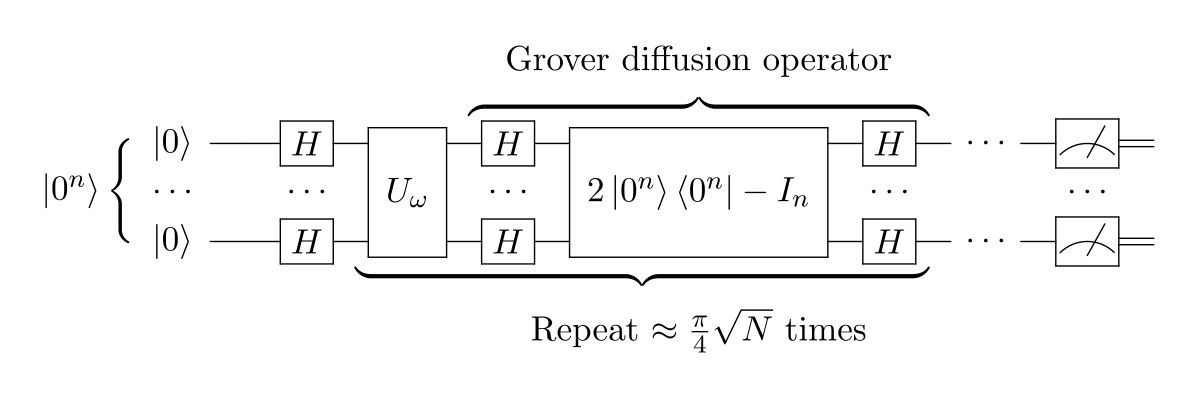
\includegraphics[width=0.8\textwidth]{05_Quantum_Impact_on_Cryptography/grovers_algorithm}
    \caption{Quantum circuit for Grover's algorithm}
    \label{fig:grover_circuit}
\end{figure}

\section{Timeline of Quantum Threat}\label{sec:timeline}

When might we expect quantum computers powerful enough to break current cryptography?  Estimates vary, but current thinking suggests that quantum computers capable of breaking RSA-2048 could potentially emerge within the next 5 to 15 years \parencite{mosca2018cybersecurity}.  However, significant hurdles remain:

\begin{itemize}
    \item \textbf{Error Correction:} Building quantum computers with sufficiently low error rates is a major technical challenge. Current error correction techniques are still imperfect \parencite{preskill2018quantum}.
    \item \textbf{Scalability:} Cryptographically relevant computations will likely require thousands of logical qubits. Scaling up current quantum computer prototypes to this size is a significant engineering undertaking.
\end{itemize}

\begin{figure}[h]
    \centering
    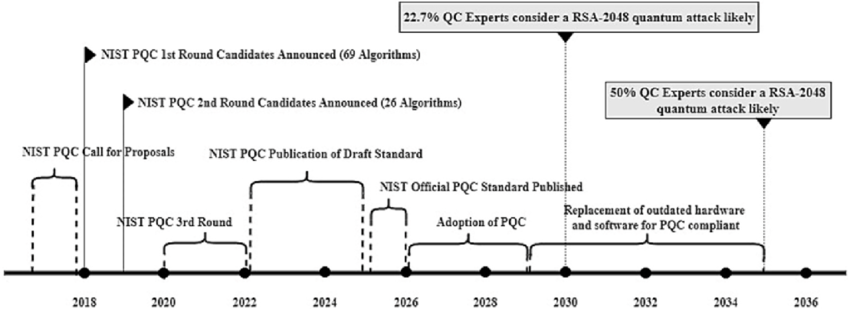
\includegraphics[width=0.8\textwidth]{06_Challenges_in_Transition/nist_timeline}
    \caption{NIST's projected timeline for quantum computer development}
    \label{fig:nist_timeline}
\end{figure}

\section{Store Now, Decrypt Later Attacks}

A significant near-term risk involves adversaries storing encrypted data now to decrypt it when quantum computers become available. This particularly threatens data with long-term value, making quantum-resistant solutions necessary even before practical quantum computers exist.

\section{Quantum-Resistant Algorithm Categories}
In response to quantum threats, cryptographers have developed several approaches to post-quantum cryptography:

\subsection{Lattice-Based Cryptography}
Lattice-based cryptosystems base their security on the hardness of certain problems in lattice theory, such as the Shortest Vector Problem (SVP) and the Learning With Errors (LWE) problem. These problems are believed to be difficult even for quantum computers. Notable examples include:
\begin{itemize}
    \item NTRU (N-th degree Truncated polynomial Ring Units)
    \item Kyber, a lattice-based key encapsulation mechanism selected by NIST for standardization
\end{itemize}

\subsection{Hash-Based Cryptography}
Hash-based signatures rely on the security of cryptographic hash functions, which are less vulnerable to quantum attacks. They include:
\begin{itemize}
    \item Merkle signature scheme
    \item XMSS (eXtended Merkle Signature Scheme), standardized by the IETF
    \item SPHINCS+, a stateless hash-based signature scheme selected by NIST
\end{itemize}

\subsection{Code-Based Cryptography}
Code-based cryptography uses error-correcting codes and derives its security from the difficulty of decoding general linear codes. McEliece, proposed in 1978, is one of the oldest post-quantum cryptographic systems and has withstood decades of cryptanalysis.

\subsection{Multivariate Polynomial Cryptography}
These systems base their security on the difficulty of solving systems of multivariate polynomials over finite fields, known to be NP-hard. Examples include the Rainbow signature scheme, though recent cryptanalysis has identified vulnerabilities in some variants.

\subsection{Isogeny-Based Cryptography}
Isogeny-based systems rely on the difficulty of finding isogenies between elliptic curves. SIKE (Supersingular Isogeny Key Encapsulation) was a notable example, though it was subsequently broken by classical attacks in 2022, highlighting the evolving nature of post-quantum cryptography research.

\section{Standardization Efforts}
The transition to quantum-resistant cryptography requires coordinated standardization efforts:

\subsection{NIST Post-Quantum Cryptography Standardization}
The U.S. National Institute of Standards and Technology launched its post-quantum cryptography standardization process in 2016. After multiple rounds of evaluation, NIST selected several algorithms for standardization in 2022:
\begin{itemize}
    \item For key encapsulation: CRYSTALS-Kyber
    \item For digital signatures: CRYSTALS-Dilithium, FALCON, and SPHINCS+
\end{itemize}

Final standards are expected to be published by 2024-2025, with additional algorithms still under consideration for future standardization.

\subsection{Other Standardization Bodies}
In parallel with NIST, other organizations are contributing to post-quantum standardization:
\begin{itemize}
    \item The Internet Engineering Task Force (IETF) is developing protocols for incorporating post-quantum algorithms into TLS and other internet standards
    \item The European Telecommunications Standards Institute (ETSI) has established a Quantum-Safe Cryptography working group
    \item The International Organization for Standardization (ISO) is developing standards for quantum-resistant cryptographic techniques
\end{itemize}

\section{Transition Challenges}
Migrating from classical to post-quantum cryptography presents significant challenges:

\subsection{Computational and Bandwidth Overhead}
Most post-quantum algorithms require larger key sizes and ciphertexts than their classical counterparts, imposing:
\begin{itemize}
    \item Increased computational demands on both servers and clients
    \item Higher bandwidth requirements for communication protocols
    \item Storage challenges for certificates and cryptographic artifacts
\end{itemize}

\subsection{Implementation and Deployment Considerations}
The transition process involves numerous practical considerations:
\begin{itemize}
    \item Identifying all systems using vulnerable cryptography
    \item Prioritizing critical infrastructure and long-term secrets
    \item Developing migration strategies that maintain backward compatibility
    \item Implementing hybrid approaches that combine classical and post-quantum algorithms during the transition period
\end{itemize}

\subsection{Cryptographic Agility}
A key lesson from the quantum threat is the importance of building cryptographic agility into systems—the ability to quickly replace cryptographic algorithms without major system overhauls. This approach provides resilience against future cryptographic vulnerabilities, whether quantum-related or otherwise.

\section{Current Industry Responses}
Major technology companies and organizations have already begun implementing quantum-resistant approaches:
\begin{itemize}
    \item Google has tested post-quantum algorithms in Chrome and other products
    \item Cloudflare has implemented experimental support for post-quantum TLS
    \item Microsoft has developed quantum-resistant VPN solutions
    \item Financial institutions are evaluating the impact on banking infrastructure and payment systems
    \item Military and intelligence agencies worldwide are prioritizing quantum-resistant encryption for classified communications
\end{itemize}

These early adoption efforts provide valuable real-world testing for post-quantum algorithms while protecting particularly sensitive systems against future quantum threats.

\section{Comparative Analysis}\label{sec:comparison}

\begin{table}[h]
    \centering
    \caption{Impact of Quantum Computing on Classical Cryptography}
    \label{tab:quantum_impact}
    \begin{tabular}{|l|c|c|}
        \hline
        \textbf{Algorithm} & \textbf{Classical Security} & \textbf{Quantum Security} \\
        \hline
        RSA-2048 & 112 bits & 0 bits \\
        AES-256 & 256 bits & 128 bits \\
        ECC-256 & 128 bits & 0 bits \\
        \hline
    \end{tabular}
\end{table}

\section{Required Security Levels}\label{sec:security_levels}

To maintain security against quantum attacks:

\begin{itemize}
    \item \textbf{Symmetric Key Algorithms:} Double the key length
    \item \textbf{Hash Functions:} Double the output length
    \item \textbf{Public Key Algorithms:} Replace with quantum-resistant alternatives
\end{itemize}

The required security level $S$ against quantum attacks is:
\begin{equation}\label{eq:quantum_security}
    S_{\text{quantum}} = \frac{S_{\text{classical}}}{2}
\end{equation}

This chapter demonstrates the urgent need for quantum-resistant cryptography, which we will explore in subsequent chapters.
\chapter{Implementation Challenges}

\section{Technical Challenges}
Implementing quantum-resistant cryptography presents several technical obstacles:

\begin{itemize}
    \item \textbf{Performance Overhead:} Post-quantum algorithms typically require more computational resources and larger key sizes than traditional cryptography
    
    \item \textbf{Resource Constraints:} Limited resources in IoT devices and embedded systems make post-quantum implementation particularly challenging
    
    \item \textbf{Side-Channel Attacks:} Some post-quantum algorithms may be vulnerable to side-channel attacks that exploit physical implementation characteristics
\end{itemize}

\section{Migration Challenges}
Transitioning to post-quantum cryptography involves significant migration hurdles:

\begin{itemize}
    \item \textbf{Legacy Systems:} Many systems with long lifespans cannot be easily updated
    
    \item \textbf{Cryptographic Inventory:} Organizations often lack complete visibility into where and how cryptography is used in their systems
    
    \item \textbf{Backward Compatibility:} Maintaining interoperability with systems that haven't yet upgraded
\end{itemize}

\section{Standardization and Deployment}
The standardization process itself poses challenges:

\begin{itemize}
    \item \textbf{Algorithm Selection:} Balancing security, performance, and implementation factors
    
    \item \textbf{Evolving Cryptanalysis:} Security assessments continue to evolve as more analysis is conducted
    
    \item \textbf{Global Adoption:} Coordinating implementation across different countries and regulatory environments
\end{itemize}

\section{Hybrid Cryptography Implementation}
Hybrid approaches combining classical and post-quantum algorithms offer a transition path:

\begin{itemize}
    \item \textbf{Protocol Modifications:} Existing protocols like TLS must be adapted to support hybrid schemes
    
    \item \textbf{Key Management Complexity:} Managing both classical and post-quantum keys adds operational complexity
\end{itemize}

\section{Testing and Validation}
Ensuring correctness and security of implementations requires:

\begin{itemize}
    \item \textbf{Test Vectors:} Standardized test inputs and outputs to verify implementations
    
    \item \textbf{Formal Verification:} Mathematical proof of algorithm implementation correctness
    
    \item \textbf{Real-World Testing:} Deployment in non-critical environments to identify practical issues
\end{itemize}

\section{Resource Planning}
Organizations need strategic approaches to post-quantum transition:

\begin{itemize}
    \item \textbf{Prioritization:} Focusing first on systems with long-term security requirements
    
    \item \textbf{Crypto-Agility:} Designing systems that can easily swap cryptographic algorithms
    
    \item \textbf{Education and Training:} Preparing technical teams to implement and manage post-quantum solutions
\end{itemize}
\chapter{Quantum-Resistant Cryptographic Solutions}\label{chap:quantum_resistant}

\section{Post-Quantum Cryptography Overview}
Post-quantum cryptography (PQC) focuses on developing algorithms that remain secure against both classical and quantum computer attacks \parencite{bernstein2017post}. Unlike current public-key systems, these next-generation approaches rely on mathematical problems believed to remain hard even for quantum computers.

\section{Lattice-Based Cryptography}\label{sec:lattice}

\subsection{Mathematical Foundations}\label{subsec:lattice_math}
Lattice-based cryptography relies on hard problems in lattice theory:

\begin{equation}\label{eq:lattice}
    L(\mathbf{B}) = \{\mathbf{Bx} : \mathbf{x} \in \mathbb{Z}^n\}
\end{equation}

where $\mathbf{B}$ is the basis matrix.

\subsection{Learning With Errors (LWE)}\label{subsec:lwe}
The LWE problem forms the basis for many quantum-resistant schemes:

\begin{equation}\label{eq:lwe}
    \mathbf{b} = \mathbf{As} + \mathbf{e} \mod q
\end{equation}

where:
\begin{itemize}
    \item $\mathbf{A}$ is a random matrix
    \item $\mathbf{s}$ is the secret vector
    \item $\mathbf{e}$ is a small error vector
\end{itemize}

\begin{itemize}
    \item \textbf{Learning With Errors (LWE):} Forms the foundation for many lattice-based systems
    \item \textbf{NTRU:} One of the earliest and most studied lattice-based systems
    \item \textbf{CRYSTALS-Kyber:} Recently selected by NIST as a standard for key encapsulation
\end{itemize}

%\begin{figure}[h]
%    \centering
%    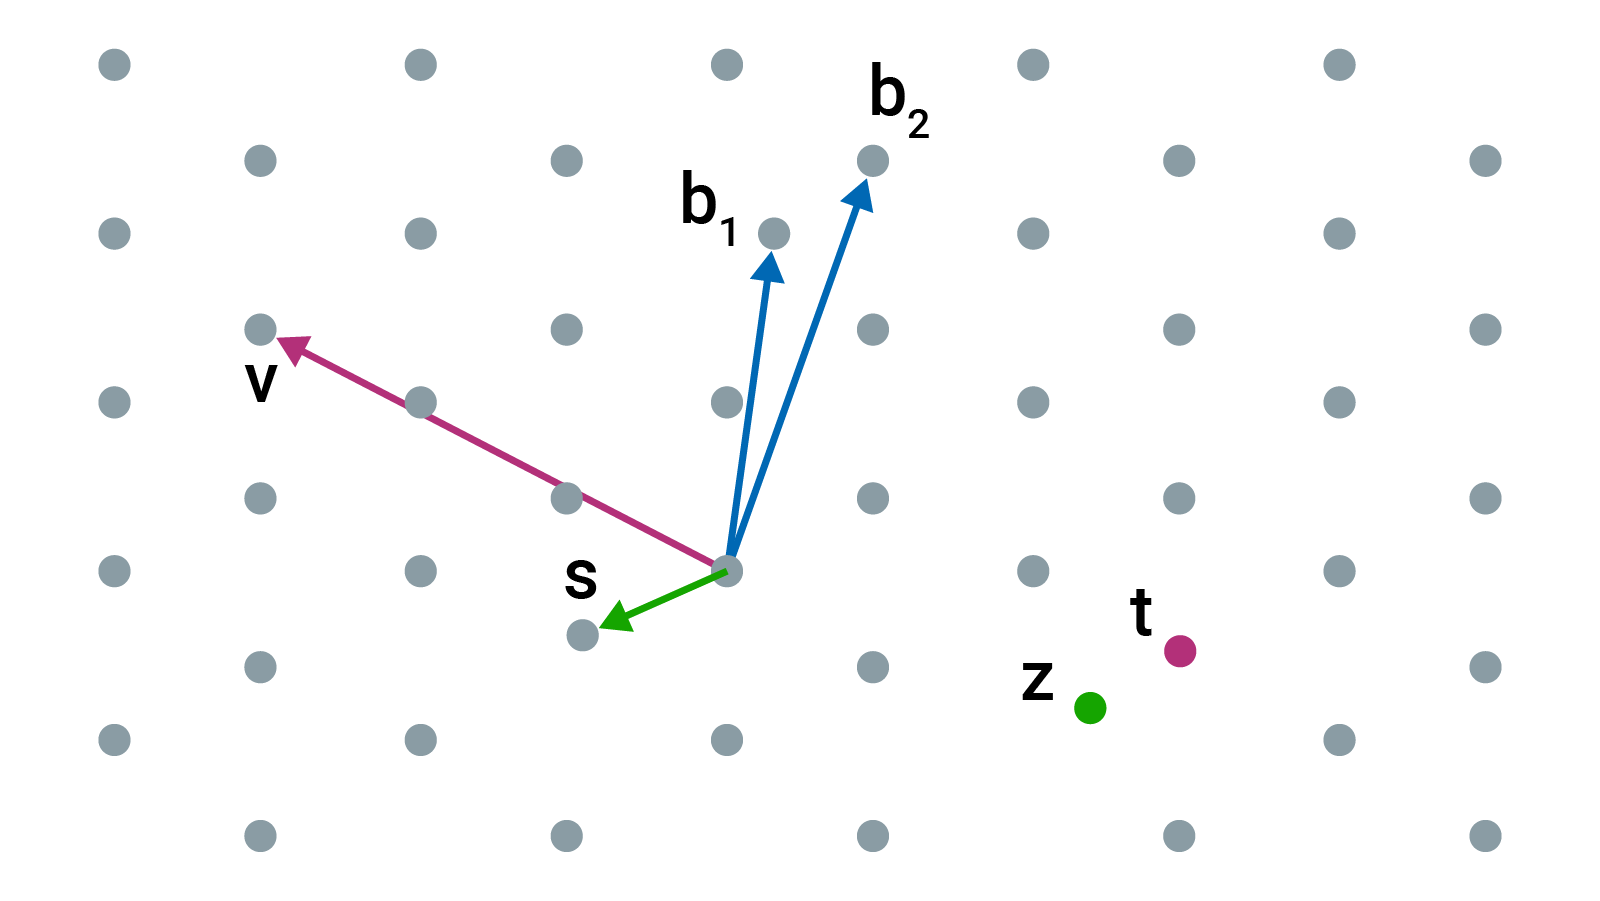
\includegraphics[width=0.7\textwidth]{lattice_cryptography.png}
%    \caption{Basic Concept of Lattice Cryptography}
%    \label{fig:lattice-crypto}
%\end{figure}

\section{Hash-Based Signatures}\label{sec:hash_based}

\subsection{Merkle Signatures}\label{subsec:merkle}
Construction of a Merkle tree:

% Commenting out missing image since merkle_tree.png is not available
%\begin{figure}[h]
%    \centering
%    \includegraphics[width=0.7\textwidth]{merkle_tree}
%    \caption{Merkle tree structure for hash-based signatures}
%    \label{fig:merkle_tree}
%\end{figure}

\subsection{SPHINCS+}\label{subsec:sphincs}
Key features of SPHINCS+:

\begin{itemize}
    \item \textbf{Security Properties:}
    \begin{itemize}
        \item Stateless design
        \item Hash-based security
        \item Forward security
    \end{itemize}
    \item \textbf{Performance Characteristics:}
    \begin{itemize}
        \item Signature size
        \item Verification speed
        \item Key generation time
    \end{itemize}
\end{itemize}

Hash-based signatures offer quantum resistance by relying solely on the security of cryptographic hash functions \parencite{bernstein2017post}. These functions are generally considered less vulnerable to quantum attacks compared to the mathematical problems underpinning traditional public-key cryptography.

\begin{itemize}
    \item \textbf{Merkle Signature Scheme:} A foundational approach using binary hash trees
    \item \textbf{SPHINCS+:} A modern, stateless hash-based signature scheme chosen by NIST
\end{itemize}

While hash-based signatures offer strong security guarantees, they typically produce larger signatures compared to traditional algorithms.

\section{Code-Based Cryptography}\label{sec:code_based}

\subsection{McEliece Cryptosystem}\label{subsec:mceliece}
The system uses error-correcting codes:

\begin{equation}\label{eq:mceliece}
    \mathbf{c} = \mathbf{mG'} + \mathbf{e}
\end{equation}

where:
\begin{itemize}
    \item $\mathbf{G'}$ is the public generator matrix
    \item $\mathbf{m}$ is the message
    \item $\mathbf{e}$ is the error vector
\end{itemize}

Code-based cryptography derives its security from the challenge of decoding general linear codes \parencite{bernstein2017post}. The McEliece system, proposed in 1978, exemplifies this approach's longevity and continued relevance in post-quantum cryptography.

\begin{itemize}
    \item \textbf{McEliece:} Has withstood decades of cryptanalysis
    \item Based on the computational difficulty of decoding linear codes
\end{itemize}

A notable characteristic of code-based systems is their requirement for larger key sizes, which can impact practical implementations.

\section{Multivariate Cryptography}\label{sec:multivariate}

\subsection{Rainbow Signature Scheme}\label{subsec:rainbow}
The multivariate quadratic system:

\begin{equation}\label{eq:rainbow}
    \mathbf{y} = \mathbf{F}(\mathbf{x}) = (f_1(\mathbf{x}), \ldots, f_m(\mathbf{x}))
\end{equation}

where each $f_i$ is a quadratic polynomial.

Multivariate cryptography is based on the difficulty of solving systems of multivariate polynomial equations:

\begin{itemize}
    \item Efficient for signatures but less practical for encryption
    \item Vulnerable to specific attacks in some implementations
\end{itemize}

\section{NIST Standardization Process}
NIST initiated its post-quantum cryptography standardization process in 2016 \parencite{alagic2020status}. After rigorous evaluation, several algorithms were selected:

\begin{itemize}
    \item \textbf{Key Encapsulation:} CRYSTALS-Kyber
    \item \textbf{Digital Signatures:} CRYSTALS-Dilithium, FALCON, and SPHINCS+
\end{itemize}

% Commenting out corrupted image
%\begin{figure}[h]
%    \centering
%    \includegraphics[width=0.7\textwidth]{post_quantum_comparison}
%    \caption{Comparison of Post-Quantum Cryptographic Approaches}
%    \label{fig:pqc-comparison}
%\end{figure}

\section{Quantum Key Distribution}
QKD takes a fundamentally different approach to security \parencite{wehner2018quantum}, leveraging quantum mechanics principles instead of mathematical complexity:

\begin{itemize}
    \item Based on the principle that measuring quantum states inevitably disturbs them
    \item Allows for the secure distribution of cryptographic keys with theoretical guarantees
    \item Requires specialized hardware and typically relies on direct optical links
    \item Currently limited to distances under 100km without quantum repeaters
\end{itemize}

\begin{figure}[h]
    \centering
    \includegraphics[width=0.6\textwidth]{06_Challenges_in_Transition/quantum_key_distribution}
    \caption{Basic Quantum Key Distribution Process}
    \label{fig:qkd-process}
\end{figure}

\section{Hybrid Approaches}\label{sec:pqc_hybrid}

\subsection{Multiple Algorithm Integration}\label{subsec:multi_algo}
Hybrid scheme security:

\begin{equation}\label{eq:pqc_hybrid_security}
    S_{\text{total}} = \min(S_{\text{classical}}, S_{\text{quantum}})
\end{equation}

During the transition to a post-quantum world, hybrid approaches offer a pragmatic path forward \parencite{bernstein2017post}:

\begin{itemize}
    \item Combine classical and post-quantum algorithms
    \item Security relies on the stronger of the two underlying schemes
    \item Provide backward compatibility with existing systems while adding quantum resistance
\end{itemize}

Companies like Google and Cloudflare have already begun experimenting with these hybrid approaches in their TLS implementations, demonstrating their practical viability.

\section{Performance Analysis}\label{sec:performance}

\begin{table}[h]
    \centering
    \caption{Performance Comparison of Post-Quantum Schemes}
    \label{tab:pq_performance}
    \begin{tabular}{|l|c|c|c|}
        \hline
        \textbf{Scheme} & \textbf{Key Size} & \textbf{Signature Size} & \textbf{Security Level} \\
        \hline
        CRYSTALS-Kyber & 1632B & N/A & 128 bits \\
        SPHINCS+ & 64B & 8080B & 128 bits \\
        Classic McEliece & 261KB & 128B & 128 bits \\
        \hline
    \end{tabular}
\end{table}

\section{Implementation Guidelines}\label{sec:pqc_implementation}

Best practices for implementing quantum-resistant cryptography:

\begin{itemize}
    \item \textbf{Algorithm Selection:}
    \begin{itemize}
        \item Security requirements
        \item Performance constraints
        \item Resource availability
    \end{itemize}
    \item \textbf{Implementation Security:}
    \begin{itemize}
        \item Side-channel protection
        \item Error handling
        \item Parameter validation
    \end{itemize}
    \item \textbf{Integration Strategy:}
    \begin{itemize}
        \item Modular design
        \item Testing framework
        \item Deployment planning
    \end{itemize}
\end{itemize}

\section{Future Considerations}\label{sec:pqc_future}

Long-term developments in quantum-resistant cryptography:

\begin{itemize}
    \item \textbf{Research Directions:}
    \begin{itemize}
        \item New mathematical problems
        \item Improved efficiency
        \item Enhanced security proofs
    \end{itemize}
    \item \textbf{Standardization:}
    \begin{itemize}
        \item NIST recommendations
        \item International standards
        \item Industry adoption
    \end{itemize}
\end{itemize}

These quantum-resistant solutions provide a foundation for securing systems against both classical and quantum threats.
\chapter{Future Prospects}
\label{chap:future-prospects}

\section{Quantum Computing Evolution}
Quantum computing will continue to develop with:
\begin{itemize}
    \item Increasing qubit counts
    \item Improved error correction
    \item More accessible quantum platforms
\end{itemize}

\section{Emerging Quantum-Resistant Techniques}
Research continues on new approaches:
\begin{itemize}
    \item Refinements to existing methods
    \item Novel mathematical foundations
    \item Combined post-quantum approaches
\end{itemize}

\section{Quantum Cryptography Advancements}
Quantum mechanics offers unique security possibilities:
\begin{itemize}
    \item Extended-range quantum key distribution
    \item Quantum repeaters for networks
    \item Device-independent protocols
\end{itemize}

\section{Research Directions}
Key research areas include:
\begin{itemize}
    \item Formal security proofs
    \item Optimization for constrained devices
    \item Migration tools for legacy systems
    \item Hardware acceleration
\end{itemize}

\section{Quantum-Safe Society}
The transition to quantum-resistant systems will create:
\begin{itemize}
    \item More resilient infrastructure
    \item Standardized cryptographic agility
    \item Hybrid classical-quantum security
\end{itemize}
\chapter{Societal Implications of Post-Quantum Cryptography}\label{chap:societal}

\section{Economic Impact}\label{sec:economic}

The transition to post-quantum cryptography will have significant economic implications:

\begin{itemize}
    \item \textbf{Infrastructure Costs:}
    \begin{itemize}
        \item Hardware upgrades
        \item Software modifications
        \item Training and implementation
    \end{itemize}
    \item \textbf{Market Opportunities:}
    \begin{itemize}
        \item New security products
        \item Consulting services
        \item Implementation expertise
    \end{itemize}
\end{itemize}

\section{Privacy and Security}\label{sec:privacy}

Long-term implications for privacy and security:

\begin{itemize}
    \item \textbf{Data Protection:}
    \begin{itemize}
        \item Historical data vulnerability
        \item Future privacy guarantees
        \item Regulatory compliance
    \end{itemize}
    \item \textbf{National Security:}
    \begin{itemize}
        \item Military communications
        \item Intelligence gathering
        \item Critical infrastructure
    \end{itemize}
\end{itemize}

\section{Digital Trust}\label{sec:trust}

Impact on trust in digital systems:

\begin{itemize}
    \item \textbf{Public Confidence:}
    \begin{itemize}
        \item Understanding of risks
        \item Trust in institutions
        \item Adoption of new systems
    \end{itemize}
    \item \textbf{Business Relations:}
    \begin{itemize}
        \item Supply chain security
        \item International trade
        \item Financial transactions
    \end{itemize}
\end{itemize}

\section{Policy Implications}\label{sec:policy}

Policy considerations for the post-quantum era:

\begin{itemize}
    \item \textbf{Regulation:}
    \begin{itemize}
        \item Compliance requirements
        \item International standards
        \item Export controls
    \end{itemize}
    \item \textbf{Government Action:}
    \begin{itemize}
        \item Research funding
        \item Infrastructure updates
        \item Public awareness
    \end{itemize}
\end{itemize}

\section{Educational Challenges}\label{sec:education}

Preparing for the post-quantum transition:

\begin{itemize}
    \item \textbf{Workforce Development:}
    \begin{itemize}
        \item Technical training
        \item Academic programs
        \item Professional certification
    \end{itemize}
    \item \textbf{Public Understanding:}
    \begin{itemize}
        \item Risk awareness
        \item Security practices
        \item Technology literacy
    \end{itemize}
\end{itemize}

\section{Global Impact}\label{sec:global}

International implications and considerations:

\begin{itemize}
    \item \textbf{Digital Divide:}
    \begin{itemize}
        \item Access to technology
        \item Implementation capacity
        \item Resource distribution
    \end{itemize}
    \item \textbf{International Cooperation:}
    \begin{itemize}
        \item Standards development
        \item Information sharing
        \item Joint research
    \end{itemize}
\end{itemize}

\section{Future Considerations}\label{sec:future}

Long-term societal considerations:

\begin{itemize}
    \item \textbf{Technological Evolution:}
    \begin{itemize}
        \item Ongoing innovation
        \item Adaptation requirements
        \item Future threats
    \end{itemize}
    \item \textbf{Social Adaptation:}
    \begin{itemize}
        \item Cultural changes
        \item Behavioral adjustments
        \item Risk perception
    \end{itemize}
\end{itemize}

\section{Recommendations}\label{sec:recommendations}

Policy and action recommendations:

\begin{enumerate}
    \item Develop comprehensive transition strategies
    \item Establish international cooperation frameworks
    \item Create public awareness programs
    \item Invest in education and training
    \item Support ongoing research and development
    \item Implement regular assessment mechanisms
\end{enumerate}

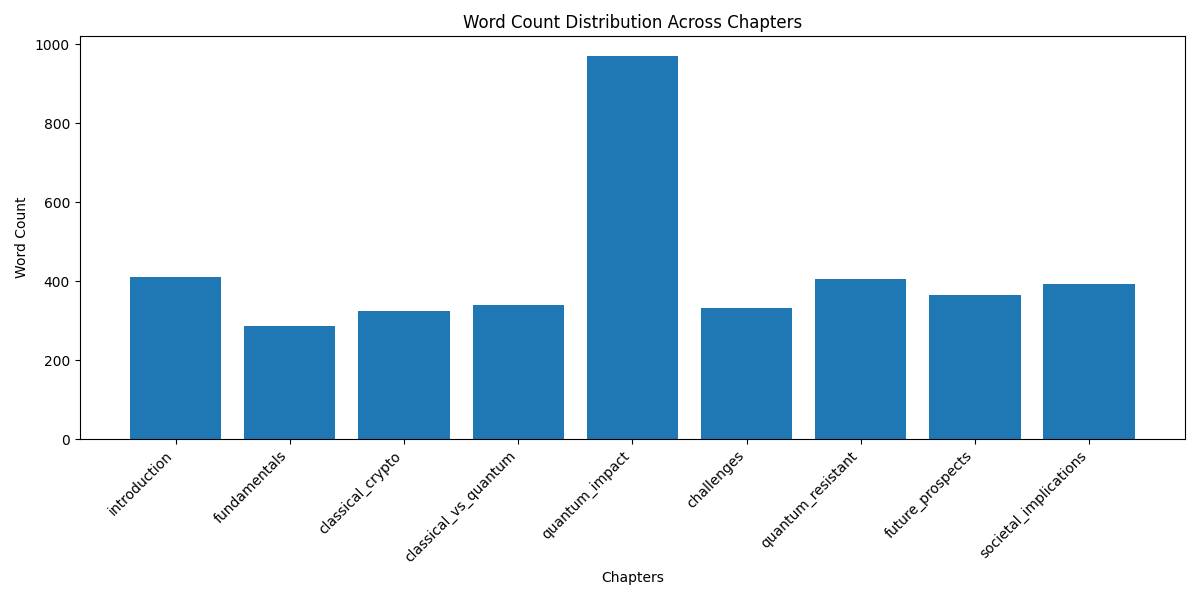
\includegraphics[width=0.8\textwidth]{09_Societal_Implications/word_distribution}

The societal implications of post-quantum cryptography extend far beyond technical considerations, requiring careful attention to economic, social, and policy dimensions to ensure a successful transition to quantum-resistant security systems.

\printbibliography[title={Sources}]

\end{document}